\documentclass[10pt]{article}
\usepackage{graphicx} % Required for inserting images
\usepackage{geometry}
\usepackage{hyperref}
\usepackage{tabularx}

\geometry{a4paper,left=20mm,right=20mm,top=20mm}
\graphicspath{{src/assets}}

\title{Relazione Progetto di Tecnologie Web}
\author{
    \textbf{2076430}\\ Gusella Manuel \and
    \textbf{2075541}\\ Marcon Giulia \and
    \textbf{2082849}\\ Perozzo Andrea \and
    \textbf{2075515}\\ Tutino Giuseppe
}
\date{A.A. 2024/25}

\begin{document}

\begin{figure}
    \centering
    
\includegraphics[width=0.5\linewidth]{logo.png}
\end{figure}
\maketitle
\renewcommand{\arraystretch}{2}
\begin{tabular}{|>{\centering\arraybackslash}m{7cm}|>{\centering\arraybackslash}m{8cm}|}
    \hline
     Link Sito Web & \url{} \\
     \hline
     E-mail referente del gruppo & manuel.gusella@studenti.unipd.it \\
    \hline
\end{tabular}

\vspace{0.5cm} 
\begin{center}
    \textbf{\Large Credenziali di accesso}
\end{center}
\vspace{0.5cm} 
\begin{tabularx}{\textwidth}{|>{\centering\arraybackslash}X|>{\centering\arraybackslash}X|>{\centering\arraybackslash}X|}
    \hline
    Ruolo & Username & Password \\
    \hline
    Utente & user & user \\
    \hline
    Amministratore & admin & admin \\
    \hline
\end{tabularx}

\newpage
\tableofcontents
\newpage

\section{Introduzione}
\subsection{Abstract}
"Doflamingo" è un marketplace digitale che contiene delle opere uniche sotto forma di NFT pubblicate direttamente dall'associazione.
Un Non-fungible token (NFT) rappresenta l'atto di proprietà e certificato di autenticità di un bene unico, in questo caso un'opera digitale. \\
Tutti i visitatori hanno la possibilità di visionare le opere e creare il proprio account digitale.\\
Gli utenti registrati possono comprare le opere, se non già possedute da qualcun'altro, attraverso una valuta digitale chiamata Ethereum (ETH). Eventualmente l'utente può decidere di vendere le opere che possiede ad altri utenti.\\ 
Inoltre gli utenti registrati possono recensire le opere dando un voto da \textbf{1 a 5 stelle}, inserendo opzionalmente anche un commento al riguardo.\\


\subsection{Analisi}
\subsubsection{Analisi del Target}
L'utenza principale sarà composta da persone appassionate agli NFT e alla loro compra-vendita. La maggioranza degli utenti non avrà un'idea precisa di ciò che vuole e per questo verrà aiutata nell'esplorazione.\\
Per impedire l'esclusione di alcune categorie si è pensato di fornire strumenti per aiutare nella ricerca degli NFT.\\
Utilizzando la metafora della pesca:
\begin{itemize}
    \item \textbf{Tiro perfetto:} L'utente sà già il nome dell'opera che vuole e potrà cercarla facilmente tramite una barra di ricerca;
    \item \textbf{Trappola per aragoste:} Grazie alla suddivisione in categorie e poter applicare ulteriori filtri sulle opere l'utente può farsi un'idea degli NFT presenti nella piattaforma.
    \item \textbf{Pesca con la rete:} La struttura del sito è semplice, quindi permette agli utenti di esplorare il sito senza sovraccarico
    \item \textbf{Boa di segnalazione:} 
\end{itemize}
\subsubsection{Utenti}
Esistono 3 tipologie di utenti:
\begin{itemize}
    \item Utente non registrato, che può eseguire le seguenti azioni:
    \begin{itemize}
        \item Visualizzare il sito con le relative opere
        \item Registrare un proprio account
        \item Autenticarsi
        \item Ricerca delle opere
        \item Visualizzare i dettagli di un'opera con le relative recensioni
    \end{itemize}
    \item Utente registrato, che può eseguire le seguenti azioni:
    \begin{itemize}
        \item Comprare le opere
        \item Recensire le opere
        \item Visualizzare le opere che possiede
        \item Vendere le opere che possiede
    \end{itemize}
    \item Amministratore, che può eseguire le seguenti azioni:
    \begin{itemize}
        \item Gestire gli utenti
        \item Aggiungere opere
        \item Visualizzare le vendite
    \end{itemize}
\end{itemize}

\section{Progettazione logica del database}

\subsection{Descrizione schema relazionale}
\begin{itemize}
    \item \textbf{utente} (\underline{username}, password, email, isAdmin, saldo)
    \item \textbf{categoria} (\underline{nome}, descrizione)
    \item \textbf{iscrizione} (\underline{\textit{utente}, \textit{categoria}})
    \item \textbf{opera} (\underline{id}, path, nome, descrizione, prezzo, \textit{possessore})
    \item \textbf{acquisto} (\underline{\textit{utente}, \textit{opera}}, prezzo, data)
    \item \textbf{appartenenza} (\underline{\textit{categoria}, \textit{opera}})
    \item \textbf{recensione} (\underline{timestamp, \textit{utente}}, commento*, \textit{opera}, voto)
\end{itemize}
Il simbolo * indica che l'attributo può essere nullo.

\subsection{Vincoli di integrità referenziale }
\begin{itemize}
    \item iscrizione.utente → utente.username
    \item iscrizione.categoria → categoria.nome
    \item opera.possessore → utente.username
    \item acquisto.utente → utente.username
    \item acquisto.opera → opera.id
    \item appartenenza.categoria → categoria.nome
    \item appartenenza.opera → opera.id
    \item recensione.utente → utente.username
    \item recensione.opera → opera.id
\end{itemize}
\subsection{Schema E-R}
\begin{center}
    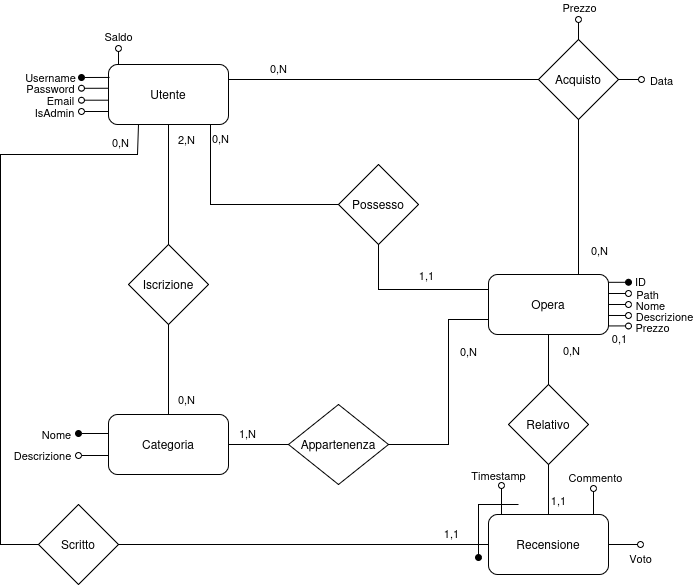
\includegraphics[width=0.6\linewidth]{schema_ristrutturato.png}
\end{center}

\section{Linguaggi}
\subsection{HTML}
Le pagine sono state create seguendo gli standard HTML5, dato che si presuppone che l'utente visiterà la pagina tramite browser più aggiornati.
\subsection{CSS}
Per rispettare la separazione tra struttura e presentazione si è deciso di utilizzare fogli di stile esterni.
\subsection{SQL}
Il sito web si appoggia su un database per le informazioni degli Utenti, delle opere, delle recensioni, degli acquisti e delle categorie.
\subsection{PHP} 
Per rispettare la separazione tra struttura e comportamento si è deciso di utilizzare script in PHP. Questi script vengono utilizzati per connettersi al database, visualizzare determinati NFT nelle pagine ed effettuare controlli di autenticazione.
\subsection{JavaScript}
JavaScript è stato utilizzato per gestire la visualizzazione dinamica dei filtri di ricerca delle pagine "NFT", "Mie recensioni", "Miei NFT" e per implementare un carosello nella sezione "Ultime uscite" della pagina Home.

\section{Progettazione}
Per la progettazione del nostro sito web, abbiamo adottato la strategia \textit{Mobile First}. Questo approccio ci ha permesso di concentrarci sulla modalità di accesso più comune per la maggioranza degli utenti, ossia quella da dispositivi mobili. Abbiamo dato priorità alla semplicità, garantendo che l’esperienza utente fosse fluida e accessibile, riducendo al minimo il numero di tap o click necessari per navigare tra le varie sezioni del sito.\\
Per il design del sito, abbiamo optato per un layout fluido, che ci ha permesso di adattare dinamicamente il layout del sito per diversi dispositivi e risoluzioni. Sebbene sia stato utilizzato un unico punto di rottura per ottimizzare l’esperienza su dispositivi mobili, il design si basa principalmente su proporzioni flessibili e sull’adattamento dei contenuti, garantendo una visualizzazione ottimale su schermi di diverse dimensioni.

\subsection{Struttura generale}
Il sito presenta una struttura semplice e lineare, senza una profondità gerarchica eccessiva. Le principali sezioni includono:
\begin{itemize}
\item \textbf{Home:} Visualizzata come landing page per accogliere l'utente che entra nel sito;
\item \textbf{NFT:} Pagina dedicata alla ricerca delle opere presenti nel sito;
\item \textbf{Singolo NFT:} Pagina che mostra i dettagli di un singolo NFT, inclusi descrizione, prezzo e recensioni degli utenti;
\item \textbf{Chi Siamo:} Pagina di presentazione dei membri del team e delle FAQ;
\item \textbf{Registrati:} Pagina per la registrazione degli utenti alla piattaforma;
\item \textbf{Login:} Pagina per l'accesso al profilo utente;
\item \textbf{Profilo:} Area personale dell'utente con informazioni personali, NFT acquistati e recensioni realizzate.
\end{itemize}

\subsection{Header e Navbar}
L'header del sito include sempre il logo, che contribuisce a definire l’identità visiva del sito.\\
La barra di navigazione è stata progettata con particolare attenzione all'accessibilità e alla semplicità, soprattutto per dispositivi mobili. Abbiamo deciso di limitare il numero di voci presenti nella navbar per eliminare la necessità di un menù ad hamburger. Questa scelta, coerente con l'approccio \textit{Mobile First}, permette agli utenti di accedere rapidamente alle informazioni desiderate senza dover compiere ulteriori tap, migliorando l’esperienza d’uso.\\
Per evitare confusione, il link alla pagina corrente viene disattivato e reso visivamente distinguibile dagli altri. Questo accorgimento aiuta a orientarsi nella navigazione senza sovraccaricare l'utente con opzioni ridondanti.\\

Sono state implementate due versioni della navbar:
\begin{itemize}
\item Per utenti non autenticati: \textbf{Home}, \textbf{NFT}, \textbf{Chi Siamo}, \textbf{Registrati}, \textbf{Accedi};
\item Per utenti autenticati: \textbf{Home}, \textbf{NFT}, \textbf{Chi Siamo}, \textbf{Profilo}, \textbf{Log out}.
\end{itemize}

\subsection{Breadcrumb}
Ogni pagina del sito include una breadcrumb che informa l'utente sulla posizione corrente all'interno della struttura del sito. Questo elemento facilita la navigazione, riducendo il rischio di disorientamento.\\
La breadcrumb segue fedelmente l’organizzazione delle pagine, mostrando i passaggi che portano alla pagina attuale. Per evitare confusione, la voce corrispondente alla pagina corrente è disattivata, eliminando il rischio di link circolari.

\subsection{Contenuto} Nella progettazione delle pagine del sito ci siamo concentrati su tre domande chiave per garantire un’esperienza utente ottimale: \begin{itemize} \item \textbf{Dove sono?} Ogni pagina presenta un chiaro titolo e, dove necessario, un breadcrumb che aiuta l’utente a comprendere la propria posizione all’interno della struttura del sito. \item \textbf{Di cosa si tratta?} Gli elementi principali di ogni pagina sono immediatamente visibili e ben distinti, con descrizioni chiare e organizzazione logica dei contenuti. \item \textbf{Dove posso andare?} I collegamenti principali sono sempre presenti nella navbar, mentre le call-to-action nelle singole pagine guidano l’utente verso le azioni principali come la ricerca, l’acquisto, o la registrazione. \end{itemize}

\subsubsection{Descrizione delle pagine} Di seguito, una panoramica delle pagine del sito:

\paragraph{Home} La home page accoglie l’utente con una breve introduzione al sito. I contenuti principali sono: \begin{itemize} \item Un carosello che mostra le 10 NFT più recenti caricate sulla piattaforma; \item Una sezione con le 3 NFT più popolari; \item Una tabella che elenca le categorie di NFT, ordinate per volume di vendite. \end{itemize} Questa struttura permette di offrire una visione sintetica e completa delle principali attività del sito.

\paragraph{Pagina NFT} Questa pagina consente agli utenti di esplorare tutte le opere disponibili sul sito. È divisa in due sezioni: \begin{itemize} \item Una form con opzioni di ricerca e filtri per affinare i risultati; \item Un elenco di NFT, organizzato in più pagine numerate (per non sovracaricare di informazioni l'utente e per rendere la pagina più veloce da caricare). \end{itemize}

\paragraph{Chi Siamo} La pagina "Chi Siamo" presenta una breve descrizione del gruppo e un elenco di domande frequenti (FAQ) che chiariscono dubbi comuni degli utenti.

\paragraph{Pagina di un singolo NFT} Questa pagina fornisce tutti i dettagli relativi a un singolo NFT. Gli elementi principali includono: \begin{itemize} \item L’immagine dell’NFT; \item Il prezzo e un pulsante per acquistarlo (visibile solo agli utenti loggati); \item Una descrizione dettagliata dell’opera; \item Una sezione per inserire una recensione (accessibile agli utenti loggati); \item L’elenco delle recensioni lasciate dagli altri utenti. \end{itemize}

\paragraph{Profilo} La pagina del profilo raccoglie le informazioni personali dell’utente. Include: \begin{itemize} \item Dati personali; \item L’elenco degli NFT acquistati dall’utente; \item Le recensioni scritte dall’utente; \item Per gli amministratori, un’opzione per aggiungere nuove NFT al sito. \end{itemize}

\paragraph{Mie Recensioni}
Questa pagina raccoglie tutte le recensioni scritte dall’utente, organizzandole in un elenco paginato per evitare problemi di scroll infinito. Ogni recensione include:
\begin{itemize} \item L’opera a cui si riferisce, con un collegamento diretto alla relativa pagina; \item Il testo completo della recensione; \item La data in cui è stata scritta la recensione.
\end{itemize} 

\paragraph{Miei NFT}
Questa pagina mostra l’elenco di tutti gli NFT acquistati dall’utente. Anche in questo caso, è stata implementata la paginazione per evitare problemi di caricamento o scroll infinito.

\paragraph{Registrati e Accedi} Queste pagine sono dedicate alla gestione degli account. Ognuna include un form semplice e diretto per la registrazione di nuovi utenti o l’accesso a un account esistente.

\paragraph{Errori 404 e 500} Per garantire un’esperienza utente coerente anche in caso di errori, le pagine 404 (pagina non trovata) e 500 (errore del server) sono state progettate con un approccio di \textit{emotional design}. Sono utilizzati messaggi rassicuranti e immagini accattivanti per ridurre il senso di frustrazione e incoraggiare l’utente a rimanere sul sito. In queste pagine, la navbar è sempre visibile e completamente funzionante, consentendo all’utente di proseguire la navigazione e mantenendo alta la fiducia dell’utente nel sito.

\subsection{Gestione della registrazione}
Il sito è navigabile senza obbligo di registrazione. Gli utenti non autenticati possono esplorare gli NFT disponibili, ma per acquistare opere o lasciare recensioni è necessaria la registrazione. Questa scelta garantisce un’esperienza più libera per l'utente, incentivando una registrazione spontanea.

\subsection{Scelta della palette colori}
La definizione della palette colori è stata un processo evolutivo, durante il quale abbiamo cambiato la palette diverse volte per garantire il contrasto minimo (4.5:1) e tenendo in considerazione che il colore di bandiera era il rosa. Inizialmente, non riuscivamo a trovare una combinazione di colori per i link che rispettasse il contrasto tra link visitati, non visitati e lo sfondo. Per risolvere il problema, abbiamo apportato leggere modifiche al colore del testo normale (da \#FFFFE8 a \#FFFEF4) e allo sfondo (da \#191919 a \#000408), in modo da aumentare il contrasto tra questi e permettere l’introduzione di un terzo colore (\#C0469D).\\
Abbiamo deciso di tenere il colore dei link non visitati identico a quello del testo normale, distinguendoli solo tramite la sottolineatura (in linea con le convenzioni esterne comunemente adottate a cui gli utenti sono abituati). Per verificare i contrasti, abbiamo utilizzato lo strumento \textit{Coolors Contrast Checker} (\url{https://coolors.co/contrast-checker/112a46-6f95bd}), ottenendo i valori richiesti.

\subsection{Accessibilità}
Per garantire un'esperienza utente ottimale, sono state adottate convenzioni che favoriscono l'usabilità e l'accessibilità del sito:
\begin{itemize}
\item Le etichette dei pulsanti e dei link sono chiare e descrittive, in modo da comunicare immediatamente l’azione associata;
\item La struttura del sito è lineare e intuitiva, con un design \textit{mobile-first} che privilegia la semplicità e l'accessibilità;
\item Il sito è navigabile tramite tastiera, garantendo l'accesso a utenti con disabilità motorie;
\item Le immagini di contenuto sono accompagnate da testi alternativi descrittivi (quando necessari), per permettere la comprensione dei contenuti da parte di utenti non vedenti o con disabilità visive;
\item Sono stati utilizzati font leggibili, con contrasto e dimensioni adeguate, per garantire la fruibilità al maggior numero di utenti possibile;
\item I contenuti interattivi sono facilmente identificabili e accessibili, con un chiaro feedback visivo per l’interazione.
\end{itemize}

\section{Implementazione}
\subsection{Front-End}
Il front-end del progetto \textit{Doflamingo} \`e stato sviluppato con l'obiettivo di fornire un'interfaccia utente intuitiva, accessibile e responsive. Per la struttura delle pagine sono stati utilizzati gli standard HTML5, mentre la presentazione grafica \`e stata curata mediante fogli di stile CSS esterni, garantendo la separazione tra contenuto e presentazione.

Le pagine includono funzionalit\`a interattive implementate attraverso JavaScript. Ad esempio, la gestione dinamica dei filtri nella ricerca degli NFT e un carosello per visualizzare le ultime opere caricate. Il design \`e stato ottimizzato per la compatibilit\`a con i principali browser moderni, offrendo un'esperienza fluida anche su dispositivi mobili.

\subsection{Back-End}
Il back-end \`e stato sviluppato utilizzando PHP per gestire la logica server-side e interagire con il database. Gli script PHP permettono di effettuare operazioni come l'autenticazione degli utenti, la gestione delle transazioni di acquisto delle opere, e la visualizzazione delle informazioni relative agli NFT e alle recensioni.

Il database \`e stato progettato utilizzando MariaDB, con una struttura relazionale che garantisce l'integrit\`a referenziale e la coerenza dei dati. Le query SQL vengono eseguite attraverso gli script PHP per recuperare, inserire e aggiornare i dati in base alle azioni dell'utente.

Per garantire una maggiore sicurezza, sono stati implementati controlli lato server degli input per prevenire vulnerabilit\`a come SQL injection e per assicurarsi che l'utente inserisca dei dati validi. Inoltre, sono state utilizzate sessioni PHP per gestire lo stato degli utenti autenticati e proteggere le operazioni sensibili.

\section{Organizzazione del lavoro}
\subsection{Gusella Manuel}
\subsection{Marcon Giulia}
\subsection{Perozzo Andrea}
\subsection{Tutino Giuseppe}

\end{document}

%  dove l'arte del futuro incontra la tecnologia blockchain..
